\documentclass{article} 
\usepackage{nips14submit_e,times}
\usepackage{hyperref}
\usepackage{url}

\usepackage{bm}
\usepackage{framed}
\usepackage{amsmath}
\usepackage{graphicx,subfig,float,amsfonts}
\usepackage{multirow}
\usepackage{array}
\usepackage{paralist}
\usepackage[numbers]{natbib}
\usepackage[algo2e,vlined,linesnumbered,algoruled]{algorithm2e}

 % preamble.tex
\usepackage{mdwlist}
\usepackage{graphicx}
\usepackage{booktabs}
\usepackage{framed}
\usepackage{color}

\newenvironment{bigenum}
{\begin{enumerate} \setlength{\itemsep}{10pt}}
{\end{enumerate}}

\newcommand{\mysec}[1]{Section~\ref{sec:#1}}
\newcommand{\myapp}[1]{Appendix~\ref{app:#1}}
\newcommand{\myeq}[1]{Equation~\ref{eq:#1}}
\newcommand{\myeqp}[1]{Eq.~\ref{eq:#1}}
\newcommand{\mychap}[1]{Chapter~\ref{chap:#1}}
\newcommand{\myfig}[1]{Figure~\ref{fig:#1}}
\newcommand{\mytab}[1]{Table~\ref{tab:#1}}

\newcommand{\g}{\,\vert\,}
\newcommand{\E}{\textrm{E}}
\newcommand{\vct}[1]{\textbf{#1}}
\newcommand{\realline}{\mathbb{R}}
\newcommand{\indpt}{\protect\mathpalette{\protect\independenT}{\perp}}
\def\independenT#1#2{\mathrel{\rlap{$#1#2$}\mkern2mu{#1#2}}}
\newcommand{\h}[1]{\textrm{H}\left( #1 \right)}
\newcommand{\half}{\frac{1}{2}}
\newcommand{\discrete}{\textrm{Discrete}}
\newcommand{\Bern}{\textrm{Bern}}
\newcommand{\DP}{\textrm{DP}}
\newcommand{\GP}{\textrm{GP}}
\newcommand{\Bet}{\textrm{Beta}}
\newcommand{\const}{\textrm{const.}}
\newcommand{\pois}{\textrm{Poisson}}
\newcommand{\ddx}[1]{\frac{\partial}{\partial #1}}
\newcommand{\dfdx}[2]{\textstyle \frac{\partial #1}{\partial #2}}
\newcommand{\yrep}{y^{\textrm{rep}}}
\newcommand{\ynew}{y^{\textrm{new}}}
\newcommand{\yobs}{y^{\textrm{obs}}}
\newcommand{\model}{\mathcal{M}}
\newcommand{\ppc}{\textrm{ppc}}
\newcommand{\ideal}{\textrm{ideal}}
\newcommand{\commentout}[1]{}
\newcommand{\comment}[1]{{\color{blue} #1}}
\newcommand{\todoL}[1]{{\color{red} Laurent please: #1}}
\newcommand{\todo}[1]{{\color{red}TODO: #1}}

\newcommand{\shape}{\textrm{shp}}
\newcommand{\rate}{\textrm{rte}}
\newcommand{\gam}{\textrm{Gamma}}
\newcommand{\vshape}[2]{\tilde{#1}_{#2}^{\shape}}
\newcommand{\vrate}[2]{\tilde{#1}_{#2}^{\rate}}


\title{Content-based recommendations\\ with Poisson factorization}
\author{
Prem Gopalan\\
Department of Computer Science\\
Princeton University\\
Princeton, NJ 08540\\
\texttt{pgopalan@cs.princeton.edu} \\
\And
Laurent Charlin\\
Department of Computer Science\\
Columbia University\\
New York, NY 10027\\
\texttt{lcharlin@cs.columbia.edu} \\
\And
David M.~Blei\\
Departments of Statistics \& Computer Science\\
Columbia University\\
New York, NY 10027\\
\texttt{david.blei@columbia.edu} \\
}

\newcommand{\fix}{\marginpar{FIX}}
\newcommand{\new}{\marginpar{NEW}}

\newcommand{\mult}{\textrm{Mult}}
\newcommand{\dirichlet}{\textrm{Dirichlet}}
\newcommand{\Gam}{\textrm{Gamma}}
\newcommand{\Pois}{\textrm{Poisson}}

\newcommand{\anon}[1]{
\ifnipsfinal 
#1
\else
anonymized for submission
\fi
}

\nipsfinalcopy 

\begin{document}

\maketitle

\begin{abstract}
We develop collaborative topic Poisson factorization (CTPF), a
generative model of articles and reader preferences. CTPF can be used
to build recommender systems by learning from reader histories and
content to recommend personalized articles of interest.  In detail,
CTPF models both reader behavior and article texts with Poisson
distributions, connecting the latent topics that represent the texts
with the latent preferences that represent the readers.  This provides
better recommendations than competing methods and gives an
interpretable latent space for understanding patterns of readership.
Further, we exploit stochastic variational inference to model massive
real-world datasets. For example, we can fit CPTF to the full arXiv
usage dataset, which contains over 43 million ratings and 42 million
word counts, within a day.  We demonstrate empirically that our model
outperforms several baselines, including the previous state-of-the art
approach.
\end{abstract}

 % intro.tex
\section{Introduction}

In this paper we develop a probabilistic model of articles and reader behavior
data. Our model is called \textit{collaborative topic Poisson factorization}
(CTPF).  It identifies the latent topics that underlie the articles, represents
readers in terms of their preferences for those topics, and captures how
documents about one topic might be interesting to the enthusiasts of another.

As a recommendation system, CTPF performs well in the face of massive,
sparse, and long-tailed data. Such data is typical because most
readers read or rate only a few articles, while a few readers may read
thousands of articles.  Further, CTPF provides a natural mechanism to
solve the ``cold start'' problem, the problem of recommending
previously unread articles to existing readers. Finally, CTPF provides
a new exploratory window into the structure of the collection. It
organizes the articles according to their topics and identifies
important articles both in terms of those important to their topic and
those that have transcended disciplinary boundaries.

We illustrate the model with an example. Consider the classic paper
"Maximum likelihood from incomplete data via the EM
algorithm"~\cite{Dempster:1977}. This paper, published in the Journal
of the Royal Statistical Society (B) in 1977, introduced the
expectation-maximization (EM) algorithm.  The EM algorithm is a
general method for finding maximum likelihood estimates in models with
hidden random variables. As many readers will know, EM has had an
enormous impact on many fields, including computer vision, natural
language processing, and machine learning. This original paper has
been cited over 37,000 times.

Figure 1 illustrates the CTPF representation of the EM paper.  (This model
was fit to the shared libraries of scientists on the Mendeley website;
the number of readers is 80,000 and the number of articles is
261,000.)  In the figure, the horizontal axes contains topics, latent
themes that pervade the collection~\cite{Blei:2003b}.  Consider the
black bars in the left figure.  These represent the topics that the EM
paper is about.  (These were inferred from the abstract of the paper.)
Specifically, it is about probabilistic modeling and statistical
algorithms.  Now consider the red bars on the right, which are summed
with the black bars.  These represent the preferences of the readers
who have the EM paper in their libraries. CTPF has uncovered the
interdisciplinary impact of the EM paper.  It is popular with readers
interested in many fields outside of those the paper discusses,
including computer vision and statistical network analysis.

The CTPF representation has advantages.  For forming recommendations,
it naturally interpolates between using the text of the article (the
black bars) and the inferred representation from user behavior data
(the red bars).  On one extreme, it recommends rarely or never read
articles based mainly on their text; this is the cold start problem.
On the other extreme, it recommends widely-read articles based mainly
on their readership.  In this setting, it can make good inferences
about the red bars.  Further, in contrast to traditional matrix
factorization algorithms, we combine the space of preferences and
articles via interpretable topics. CTPF thus offers reasons for making
recommendations, readable descriptions of reader preferences, and an
interpretable organization of the collection.  For example, CTPF can
recognize the EM paper is among the most important statistics papers
that has had an interdisciplinary impact.

In more detail, CTPF draws on ideas from two existing models:
collaborative topic regression~\cite{Wang:2011a} and Poisson
factorization~\cite{Gopalan:2013b}.  Poisson factorization is a form
of probabilistic matrix factorization~\cite{Salakhutdinov:2008} that
replaces the usual Gaussian likelihood and real-valued representations
with a Poisson likelihood and non-negative representations.  Compared
to Gaussian factorization, Poisson factorization enjoys more efficient
inference and better handling of sparse data.  However, PF is a basic
recommendation model. It cannot handle the cold start problem or
easily give topic-based representations of readers and articles.

Collaborative topic regression is a model of text and reader data that
is based on the same intuitions as we described above.  (\citet{Wang:2011a}
also use the EM paper as an example.)  However,
in its implementation, collaborative topic regression is a
non-conjugate model that is complex to fit, difficult to work with on
sparse data, and difficult to scale without stochastic optimization.
Further, it is based on a Gaussian likelihood of reader behavior.
Collaborative Poisson factorization, because it is based on Poisson
and gamma variables, enjoys an easier-to-implement and more efficient
inference algorithm and a better fit to sparse real-world data.  As we
show below, it scales more easily and provides significantly better
recommendations than collaborative topic regression.


 % model.tex
\section{The collaborative topic Poisson factorization model}
\label{sec:model}
In this section we describe the collaborative topic Poisson
factorization model~(CTPF), and discuss its statistical properties. We
are given data about users (readers) and documents (articles), where
each user has read or placed in his library a set of documents. The
rating $r_{ud}$ equals one if user $u$ consulted document $d$, can be
greater than zero if the user rated the document and is zero
otherwise.  Most of the values of the matrix $y$ are typically zero,
due to sparsity of user behavior data.

\begin{figure*}[t!]
\centering
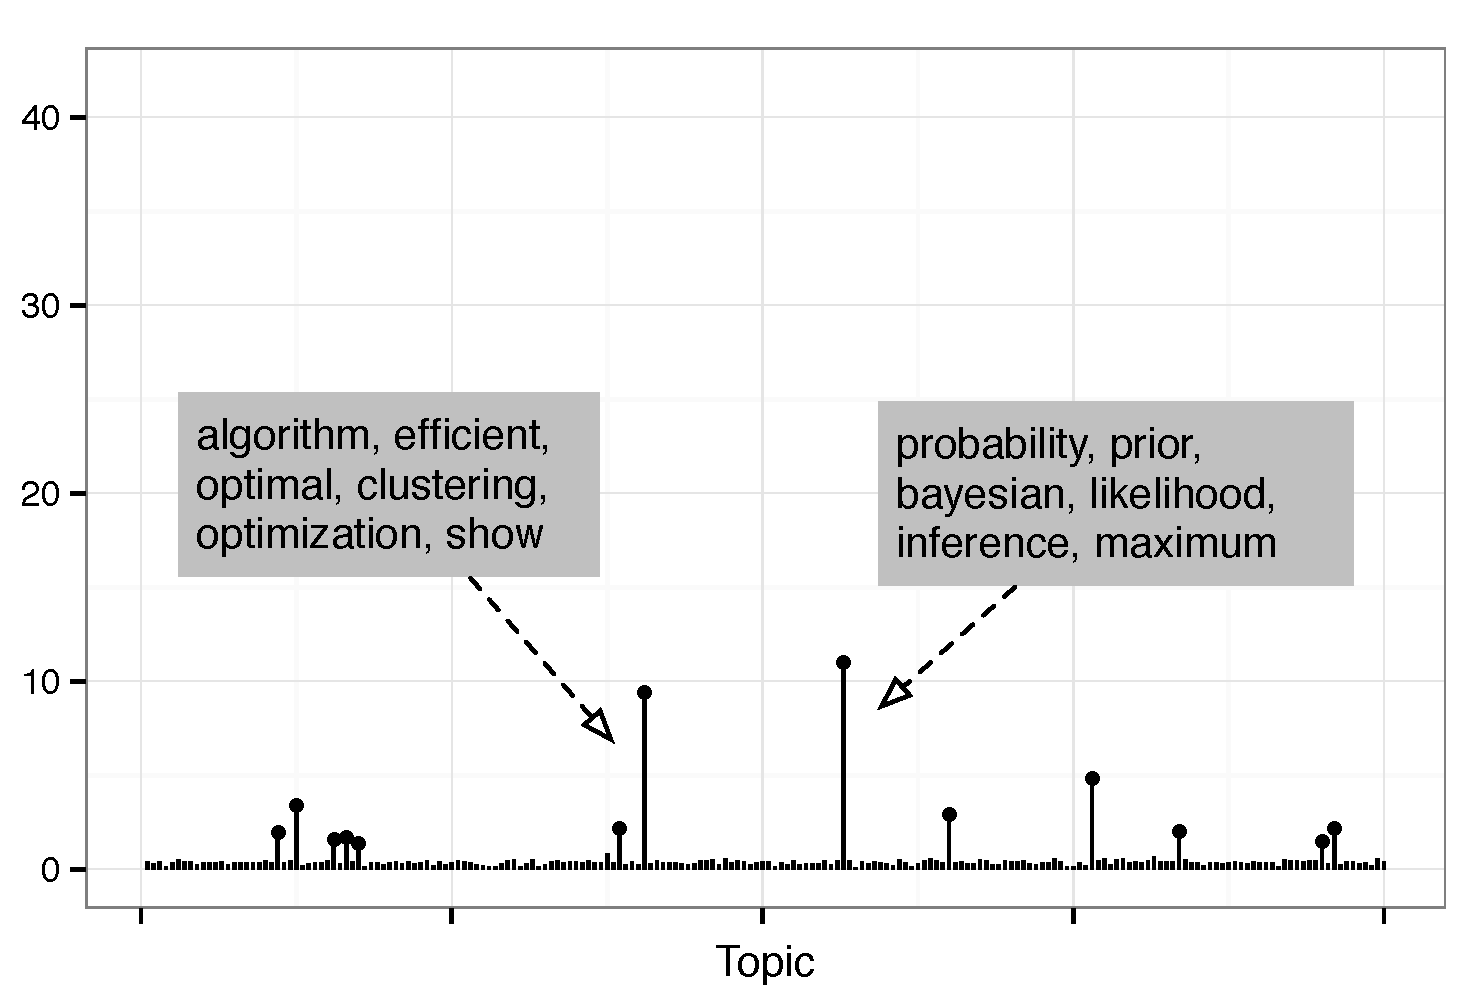
\includegraphics[width=0.48\textwidth]{../fig/pdf/em_algorithm1.pdf}
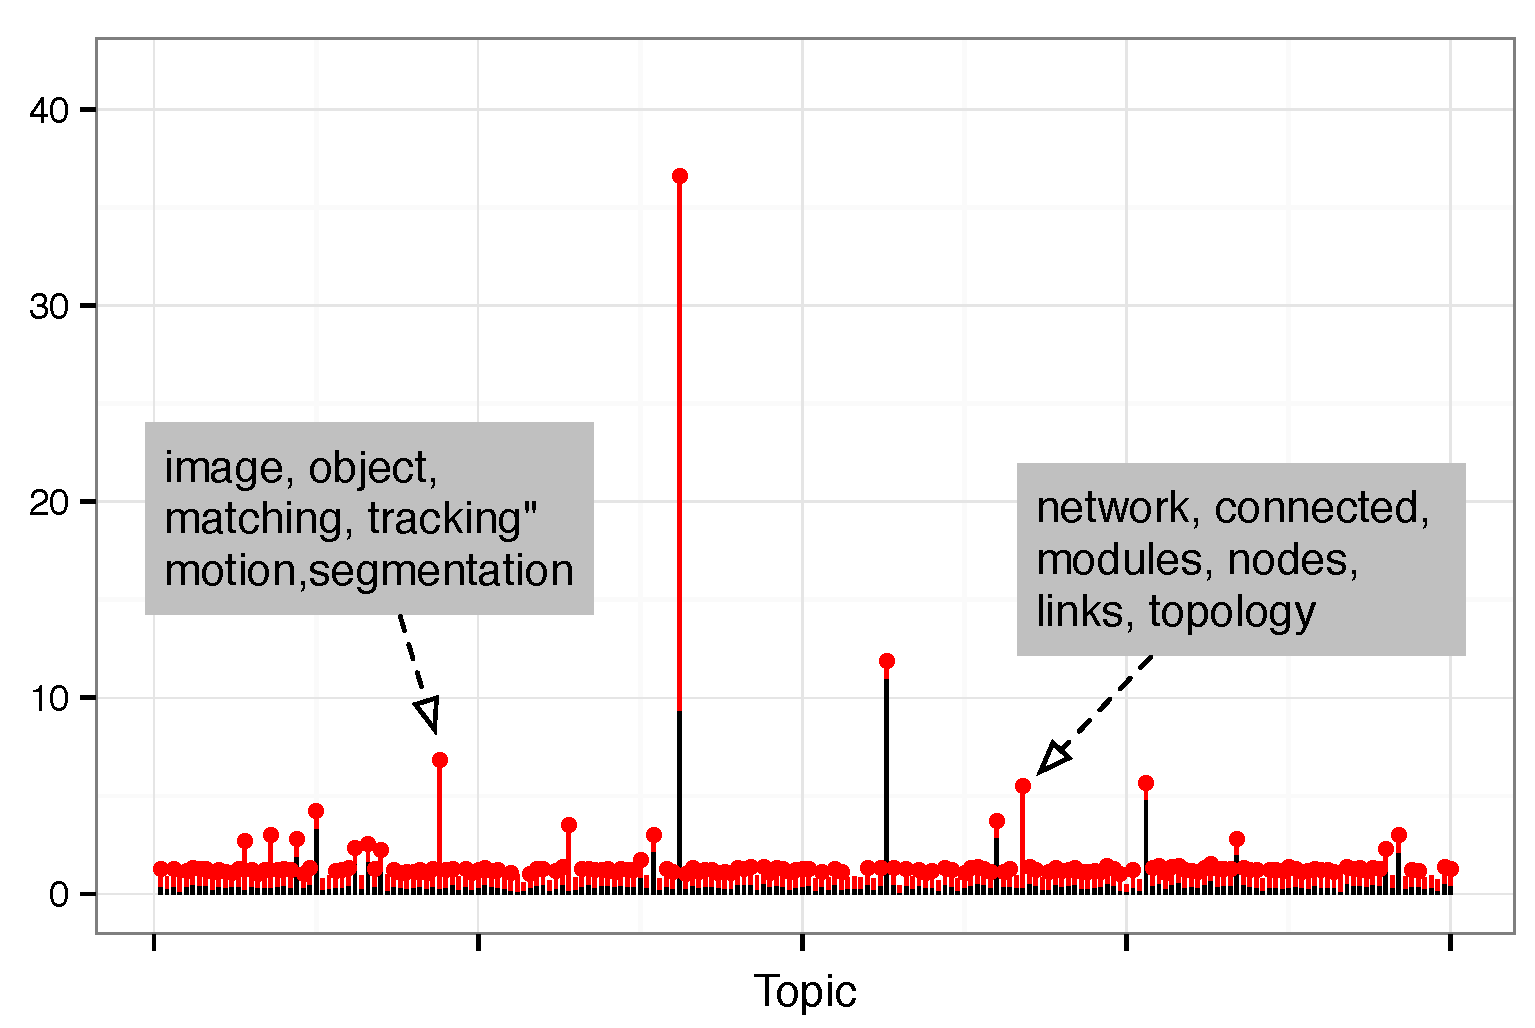
\includegraphics[width=0.48\textwidth]{../fig/pdf/em_algorithm2.pdf}\\
\caption{We visualized the inferred topic intensities $\theta$ (the
  black bars) and the topic offsets $\epsilon$ (the red bars) of an
  article in the Mendeley~\cite{Jack:2010} dataset.  The plots are for
  the statistics article titled ``Maximum likelihood from incomplete
  data via the EM algorithm''.  The black bars represent the topics
  that the EM paper is about. These include probabilistic modeling and
  statistical algorithms. The red bars represent the preferences of
  the readers who have the EM paper in their libraries. It is popular
  with readers interested in many fields outside of those the paper
  discusses, including computer vision and statistical network
  analysis.}

\label{fig:em_alg}
\end{figure*}

\paragraph{Background: Poisson factorization.} 
CTPF builds on Poisson matrix factorization~\cite{Gopalan:2013b}. In
collaborative filtering, Poisson factorization (PF) is a probabilistic
model of users and items. It associates each user with a latent vector
of preferences, each item with a latent vector of attributes, and
constrains both sets of vectors to be sparse and non-negative. Each
cell of the observed matrix is assumed drawn from a Poisson
distribution, whose rate is a linear combination of the corresponding
user and item attributes. Poisson factorization has also been used as
a topic model~\cite{Canny:2004}, and developed as an alternative text
model to latent Dirichlet allocation (LDA). In both applications
Poisson factorization has been shown to outperform competing
methods~\cite{Canny:2004, Gopalan:2013b}.  PF is also more easily
applicable to real-life preference datasets than the popular Gaussian
matrix factorization~\cite{Gopalan:2013b}. 

\paragraph{Collaborative topic Poisson factorization.} 
CTPF is a latent variable model of user ratings and document content.
CTPF uses Poisson factorization to model both types of data. Rather
than modeling them as independent factorization problems, we connect
the two latent factorizations using a correction
term~\cite{Wang:2011a} which we'll describe below.

Suppose we have data containing $D$ documents and $U$ users. CTPF
assumes a collection of $K$ unormalized \emph{topics} $\beta_{1:K}$. Each topic
$\beta_k$ is a collection of word intensities on a vocabulary of size
$V$. Each component $\beta_{vk}$ of the unnormalized topics is drawn
from a Gamma distribution. Given the topics, CTPF assumes that a
document $d$ is generated with a vector of $K$ latent \emph{topic
  intensities} $\theta_d$, and represents users with a vector of $K$
latent \emph{topic preferences} $\eta_u$.  Additionally, the model
associates each document with $K$ latent \emph{topic offsets}
$\epsilon_d$ that capture the document's deviation from the topic
intensities. These deviations occur when the content of a document is
insufficient to explain its ratings. For example, these variables can
capture that a machine learning article is interesting to a biologist,
because other biologists read it.

We now define a generative process for the observed word counts in
documents and observed user ratings of documents under CTPF:
\begin{enumerate}
\item {\bf Document model:}
\begin{enumerate}
\item Draw topics $\beta_{vk} \sim \Gam(a, b)$
\item Draw document topic intensities $\theta_{dk} \sim \Gam(c, d)$
\item Draw word count $w_{dv} \sim \Pois(\theta_d^T \beta_v)$.
\end{enumerate}

\item {\bf Recommendation model:}
\begin{enumerate}
\item Draw user preferences $\eta_{uk} \sim \Gam(e, f)$
\item Draw document topic offsets $\epsilon_{dk} \sim \Gam(g, h)$
\item Draw $r_{ud} \sim \Pois(\eta_u^T (\theta_d + \epsilon_d))$.
\end{enumerate}
\end{enumerate}

CTPF specifies that the conditional probability that a user $u$ rated
document $d$ with rating $r_{ud}$ is drawn from a Poisson distribution
with rate parameter $\eta_u^T (\theta_d + \epsilon_d)$. The form of
the factorization couples the user preferences for the document topic
intensities $\theta_d$ and the document topic offsets
$\epsilon_d$. This allows the user preferences to be interpreted as
affinity to latent topics.

CTPF has two main advantages over previous work (e.g., \cite{Wang:2011a}), both of which contribute to its superior
empirical performance (see \mysec{eval}). First, CTPF is a
conditionally conjugate model when augmented with auxiliary
variables. This allows CTPF to conveniently use standard variational
inference with closed-form updates (see \mysec{inference}). Second,
CTPF is built on Poisson factorization; it can take advantage of the
natural sparsity of user consumption of documents and can analyze
massive real-world data. This follows from the likelihood of the
observed data under the model~\cite{Gopalan:2013b}.

We analyze user preferences and document content with CTPF via its
posterior distribution over latent variables $p(\beta_{1:K},
\theta_{1:D}, \epsilon_{1:D}, \eta_{1:U} | \bm{w}, \bm{r})$. By
estimating this distribution over the latent structure, we can
characterize user preferences and document readership in many useful
ways. \myfig{em_alg} gives an example.

\commentout{
Figure 1 gives an example. The plots visualize the estimated topic intensities
and the topic offsets for two articles in the Mendeley dataset. We analyzed
the full dataset consisting of 80,000 articles and 260,000 readers, and
selected two popular articles, one each in the fields of Optimization and
Statistics. Each article exhibits topic intensities relevant to its main field,
but the topic offsets reveal the readership in external fields.  The classic
statistics article in Figure 1 exhibits ``Algorithms'' and ``Bayesian
inference'' topics, but the user library patterns reveal interest from a wide
range of scientists, including scientists who work in the fields of ``Image
processing'' and ``Networks''. 
}

\paragraph{Recommending old and new documents.}
Once the posterior is fit, we use CTPF to recommend \emph{in-matrix}
documents and \emph{out-matrix} or \emph{cold-start} documents to
users. We define in-matrix documents as those that have been rated by
at least one user in the recommendation system.  All other documents
are new to the system. A cold-start recommendation of a new document
is based entirely on its content. For predicting both in-matrix and
out-matrix documents, we rank each user's unread documents by their
posterior expected Poisson parameters,
\begin{align}
\text{score}_{ud} = \E [ \eta_u^T (\theta_d + \epsilon_d) | \bm{w}, \bm{r} ].
\end{align}
The intuition behind the CTPF posterior is that when there is no
reader data, we depend on the topics to make recommendations. When
there is both reader data and article content, this gives information
about the topic offsets. We emphasize that under CTPF the in-matrix
recommendations and cold-start recommendations are not disjoint
tasks. There is a continuum between these tasks. For example, the
model can provide better predictions for articles with few ratings by
leveraging its latent topic intensities $\theta_d$.\looseness=-1


 % inference.tex
\section{Approximate posterior inference}
\label{sec:inference}
Given a set of observed document ratings $\bm{r}$ and their word
counts $\bm{w}$, our goal is to infer the topics $\beta_{1:K}$, the
user preferences $\eta_{1:U}$, the document topic intensities
$\theta_{1:D}$, the document topic offsets $\epsilon_{1:D}$. With
estimates of these quantities, we can recommend in-matrix and
out-matrix documents to users.

Computing the exact posterior distribution $p(\beta_{1:K},
\theta_{1:D}, \epsilon_{1:D}, \eta_{1:U} | \bm{w}, \bm{r})$ is
intractable; we use variational inference~\cite{Jordan:1999}. We first
develop a coordinate ascent algorithm---a batch algorithm that
iterates over only the non-zero document-word counts and the non-zero
user-document ratings. We then present a more scalable stochastic
variational inference algorithm.

In variational inference we first define a parameterized family of
distributions over the hidden variables. We then fit the parameters to
find a distribution that minimizes the KL divergence to the
posterior. The model is conditionally conjugate if the complete
conditional of each latent variable is in the exponential family and
is in the same family as its prior. (The complete conditional is the
conditional distribution of a latent variable given the observations
and the other latent variables in the model~\cite{Ghahramani:2000}.)
For the class of conditionally conjugate models, we can perform this
optimization with a coordinate ascent algorithm and closed form updates.

\paragraph{Auxiliary variables.} To facilitate inference, we first augment
CTPF with auxiliary variables. Following Ref.~\cite{Dunson:2005} and
Ref.~\cite{Gopalan:2013b}, we add $K$ latent variables $z_{dv,k} \sim
\Pois(\theta_{dk} \beta_{vk})$, which are integers such that $w_{dv} =
\sum_k z_{dv,k}$.  Similarly, for each observed rating $r_{ud}$, we
add $K$ latent variables $y_{ud,k}^a \sim \Pois(\eta_{uk}
\theta_{dk})$ and $K$ latent variables $y_{ud,k}^b \sim
\Pois(\eta_{uk} \epsilon_{dk})$ such that $r_{ud} = \sum_k y_{ud,k}^a
+ y_{ud,k}^b$. A sum of independent Poisson random variables is itself
a Poisson with rate equal to the sum of the rates. Thus, these new
latent variables preserve the marginal distribution of the
observations, $w_{dv}$ and $r_{ud}$.
Further, when the observed counts are 0, these auxiliary variables are
not random. Consequently, our inference procedure need only consider
the auxiliary variables for non-zero observations.

CTPF with the auxiliary variables is conditionally conjugate; its
complete conditionals are shown in \mytab{conditionals}. The complete
conditionals of the Gamma variables $\beta_{vk}$, $\theta_{dk}$,
$\epsilon_{dk}$, and $\eta_{uk}$ are Gamma distributions with shape
and rate parameters as shown in \mytab{conditionals}. For the
auxiliary Poisson variables, observe that $z_{dv}$ is a
$K$-dimensional latent vector of Poisson counts, which when
conditioned on their observed sum $w_{dv}$, is distributed as a
multinomial~\cite{Johnson:2005, Cemgil:2009}. A similar reasoning
underlies the conditional for $y_{ud}$ which is a $2K$-dimensional
latent vector of Poisson counts.  With our complete conditionals in
place, we now derive the coordinate ascent algorithm for the expanded
set of latent variables.

\begin{table*}[t]
\begin{center}
\begin{small}
\begin{tabular}{llll}
\toprule
Latent Variable & Type & Complete conditional & Variational parameters\\
\midrule
$\theta_{dk}$ & $\Gam$ & $c + \sum_v z_{dv,k} + \sum_u y_{ud,k}^a, d + \sum_v
\beta_{vk} + \sum_u \eta_{uk}$ & $\vshape{\theta}{dk}, \vrate{\theta}{dk}$ \\
$\beta_{vk}$ & $\Gam$ & $a + \sum_d z_{dv,k}, b + \sum_d \theta_{dk}$ &
$\vshape{\beta}{vk}, \vrate{\beta}{vk}$\\
$\eta_{uk}$ & $\Gam$ & $e + \sum_d y_{ud,k}^a + \sum_d
y_{ud,k}^b, f + \sum_d (\theta_{dk} + \epsilon_{dk})$& $\vshape{\eta}{uk}, \vrate{\eta}{uk}$\\
$\epsilon_{dk}$ & $\Gam$ & $g + \sum_u y_{ud,k}^b, h + \sum_u \eta_{uk}$ &
$\vshape{\epsilon}{dk}, \vrate{\epsilon}{dk}$\\
$z_{dv}$ & $\mult$ & $\log \theta_{dk} + \log \beta_{vk}$ & $\phi_{dv}$\\
$y_{ud}$ & $\mult$ & $\begin{cases} 
  \log \eta_{uk} + \log \theta_{dk} \quad \text{if $k < K$},\\
  \log \eta_{uk} + \log \epsilon_{dk} \quad \text{if $K \le k < 2K$}
\end{cases}$ & $\xi_{ud}$\\
\bottomrule
\end{tabular}
\end{small}
\end{center}
\caption{CTPF: latent variables, complete conditionals and variational parameters.}
\label{tab:conditionals}
\end{table*}

\paragraph{Variational family.}
We define the mean-field variational family
$q(\beta,\theta,\eta,\epsilon,z,y)$ over the latent variables where
we consider these variables to be independent and each governed by its
own distribution,
\begin{align}
  q(\beta, \theta, \epsilon, \eta, z, y) =& 
  \prod_{v,k} q(\beta_{vk}) \prod_{d,k}
  q(\theta_{dk}) q(\epsilon_{dk}) \prod_{u,k} q(\eta_{uk}) \prod_{ud,k}
  q(y_{ud,k}) \prod_{dv,k} q(z_{dv,k}).
  \label{eq:vfamily}
\end{align}

The variational factors for topic components $\beta_{vk}$, topic
intensities $\theta_{dk}$, user preferences $\eta_{uk}$ are all Gamma
distributions---the same as their conditional distributions---with
freely set shape and rate variational parameters. For example, the
variational distribution for the topic intensities $\theta_{dk}$ is
$\gam(\theta_{dk}; \vshape{\theta}{dk}, \vrate{\theta}{dk})$. We
denote shape with the superscript ``shp'' and rate with the
superscript ``rte''. The variational factor for $z_{dv}$ is a
multinomial $\mult(w_{dv}, \phi_{dv})$ where the variational parameter
$\phi_{dv}$ is a point on the $K$-simplex. The variational factor for
$y_{ud} = (y_{ud}^a,y_{ud}^b)$ is also a multinomial $\mult(r_{ud},
\xi_{ud})$ but here $\xi_{ud}$ is a point in the $2K$-simplex.

\paragraph{Optimal coordinate updates.}
In coordinate ascent we iteratively optimize each variational
parameter while holding the others fixed. Under the conditionally
conjugate augmented CTPF, we can optimize each coordinate in closed
form by setting the variational parameter equal to the expected
natural parameter (under $q$) of the complete conditional. For a given
random variable, this expected conditional parameter is the
expectation of a function of the other random variables and
observations. (For details, see ~\cite{Gopalan:2013b,
  Hoffman:2013}). We now describe two of these updates; the other
updates are similarly derived.

The update for the variational shape and rate parameters of topic
intensities $\theta_{dk}$ is
\begin{eqnarray}
  \tilde{\theta}_{dk} &=& \langle c + \textstyle \sum_{v} w_{dv}
  \phi_{dv,k} + \sum_{u} r_{ud} \xi_{ud,k},
  d + \textstyle \sum_v \frac{\vshape{\beta}{vk}}{\vrate{\beta}{vk}} + \sum_u
  \frac{\vshape{\eta}{uk}}{\vrate{\eta}{uk}} \rangle.
\label{eq:gamma-up}
\end{eqnarray}
The Gamma update in \myeq{gamma-up} derives from the expected natural
parameter (under q) of the complete conditional for $\theta_{dk}$ in
\mytab{conditionals}. In the shape parameter for topic intensities for
document $d$, we use that $\E_q[z_{dv,k}] = w_{dv} \phi_{dv,k}$ for
the word indexed by $v$ and $\E_q[y_{ud,k}^{a}] = r_{ud}\xi_{ud,k}$
for the user indexed by $u$. In the rate parameter, we use that the
expectation of a Gamma variable is the shape divided by the rate.

The update for the multinomial $\phi_{dv}$ is
\begin{eqnarray}
  \phi_{dv} & \propto & \exp\{\Psi(\vshape{\theta}{dk}) - \log \vrate{\theta}{dk}
+ \Psi(\vshape{\beta}{vk}) - \log \vrate{\beta}{vk} \},
\label{eq:mult-up}
\end{eqnarray}
where $\Psi(\cdot)$ is the digamma function (the first derivative of
the log $\Gamma$ function).  This update comes from the expectation of
the log of a Gamma variable, for example, $\E_q[\log \theta_{dk}] =
\Psi(\vshape{\theta}{dk}) - \log \vrate{\theta}{dk}$.

\paragraph{Coordinate ascent algorithm.}
The CTPF coordinate ascent algorithm is illustrated in
\myfig{batch}. Similar to the algorithm of~\cite{Gopalan:2013b}, our
algorithm is efficient on sparse matrices. In steps 1 and 2, we need to only
update variational multinomials for the non-zero word counts $w_{dv}$
and the non-zero ratings $r_{ud}$.  In step 3, the sums over
the expected $z_{dv,k}$ and the expected $y_{ud,k}$ need only to
consider non-zero observations. This efficiency comes from the
likelihood of the full matrix depending only on the non-zero
observations~\cite{Gopalan:2013b}.
\begin{figure}
\begin{framed}
Initialize the topics $\beta_{1:K}$ and topic intensities
$\theta_{1:D}$ using LDA~\cite{Blei:2003b} as described in
\mysec{inference}.\\ Repeat until convergence:
\begin{enumerate}
\item For each word count $w_{dv} > 0$, set $\phi_{dv}$ to the expected
  conditional parameter of $z_{dv}$.
\item For each rating $r_{ud} > 0$, set $\xi_{ud}$ to the expected
  conditional parameter of $y_{ud}$.
\item For each document $d$ and each $k$, update the block of
  variational topic intensities $\tilde{\theta}_{dk}$ to their
  expected conditional parameters using \myeq{gamma-up}. Perform
  similar block updates for $\tilde{\beta}_{vk}$, $\tilde{\eta}_{uk}$
  and $\tilde{\epsilon}_{dk}$, in sequence.
\end{enumerate}
\end{framed}
\caption{The CTPF coordinate ascent algorithm. The expected
  conditional parameters of the latent variables are computed from
  \mytab{conditionals}.}
\label{fig:batch}
\end{figure}

\paragraph{Stochastic algorithm.}
The CTPF coordinate ascent algorithm is efficient: it only iterates
over the non-zero observations in the observed matrices. The algorithm
computes approximate posteriors for datasets with ten million
observations within hours (see \mysec{eval}). To fit to larger
datasets, within hours, we develop an algorithm that subsamples a
document and estimates variational parameters using stochastic
variational inference~\cite{Hoffman:2013}. The stochastic algorithm is
also useful in settings where new items continually arrive in a
stream. The CTPF SVI algorithm is described in the Appendix.
 
\paragraph{Computational efficiency.} 
The SVI algorithm is more efficient than the batch algorithm. The
batch algorithm has a per-iteration computational complexity of $O((W
+ R)K)$ where $R$ and $W$ are the total number of non-zero
observations in the document-user and document-word matrices,
respectively. For the SVI algorithm, this is $O((w_d+r_d)K)$ where
$r_d$ is the number of users rating the sampled document $d$ and $w_d$
is the number of unique words in it. (We assume that a single document
is sampled in each iteration.) In \myfig{batch}, the sums involving
the multinomial parameters can be tracked for efficient memory
usage. The bound on memory usage is $O((D+V+U)K)$.

\textbf{Hyperparameters, initialization and stopping criteria:}
Following~\cite{Gopalan:2013b}, we fix each Gamma shape and rate
hyperparameter at 0.3. We initialize the variational parameters for
$\eta_{uk}$ and $\epsilon_{dk}$ to the prior on the corresponding
latent variables and add small uniform noise. We initialize
$\tilde{\beta}_{vk}$ and $\tilde{\theta}_{dk}$ using estimates of their normalized
counterparts from LDA~\cite{Blei:2003b} fitted to the document-word
matrix $\bm{w}$. For the SVI algorithm described in the Appendix, we
set learning rate parameters $\tau_0=1024,\kappa=0.5$ and use a
mini-batch size of 1024. In both algorithms, we declare convergence
when the change in expected predictive likelihood is less than
0.001\%.


 % related.tex
\section{Related work}
\label{sec:related}

Several research efforts propose joint models of item covariates and
user activity. \citet{Singh:2008} present a framework for
simultaneously factorizing related matrices, using generalized link
functions and coupled latent spaces. \citet{Hong:2013} propose
Co-factorization machines for modeling user activity on twitter with
tweet features, including content. They study several design choices
for sharing latent spaces. While CTPF is roughly an instance of these
frameworks, we focus on the task of recommending articles to readers.

\citet{Agarwal:2010} propose fLDA, a latent factor model which
combines document features through their empirical
LDA~\cite{Blei:2003b} topic intensities and other covariates, to
predict user preferences. The coupling of matrix decomposition and
topic modeling through shared latent variables is also considered in
\cite{Shan:2010,Zhang:2012}. Like fLDA, both papers tie latent spaces
without corrective terms. \citet{Wang:2011a} have shown the importance
of using corrective terms through the collaborative topic regression
(CTR) model which uses a latent topic offset to adjust a document's
topic proportions. CTR has been shown to outperform a variant of
fLDA~\cite{Wang:2011a}. Our proposed model CTPF uses the CTR approach
to sharing latent spaces.

CTR~\cite{Wang:2011a} combines topic modeling using
LDA~\cite{Blei:2003b} with Gaussian matrix factorization for one-class
collaborative filtering~\cite{Hu:2008}. Like CTPF, the underlying MF
algorithm has a per-iteration complexity that is linear in the number
of non-zero observations. Unlike CTPF, CTR is not conditionally
conjugate, and the inference algorithm depends on numerical
optimization of topic intensities. Further, CTR requires setting
confidence parameters that govern uncertainty around a class of
observed ratings. As we show in \mysec{eval}, CTPF scales more easily
and provides significantly better recommendations than CTR.

. 


 % eval.tex
\vspace{-0.7cm}
\section{Empirical results}
\label{sec:eval}
We use the predictive approach to evaluating model
fitness~\cite{Geisser:1979}, comparing the predictive accuracy of the
CTPF coordinate ascent algorithm in \myfig{batch} to collaborative
topic regression (CTR)~\cite{Wang:2011}. We also compare to variants
of CTPF to demonstrate that coupling the latent spaces using
corrective terms is essential for good predictive performance, and
that CTPF predicts significantly better than its variants and
CTR. Finally, we explore large real-world data sets revealing the
interaction patterns between readers and articles.

\paragraph{Data sets.} We study the CTPF algorithm of \myfig{batch} on
two data sets.  The {\bf Mendeley} data set~\cite{Jack:2010} of
scientific articles is a binary matrix of 80,000 users and 260,000
articles with 5 million observations. Each cell corresponds to the
presence or absence of an article in a scientist's online library. The
{\bf arXiv} data set is a matrix of 120,297 users and 825,707
articles, with 43 million observations. Each observation indicates
whether or not a user has consulted an article (or its abstract). This
data was collected from the access logs of registered users on the
http://arXiv.org paper repository.  The articles and the usage data
spans a timeline of 10 years (2003-2012).  In our experiments on
predictive performance, we use a subset of the data set, with 64,978
users 636,622 papers and 7.6 million clicks, which spans one year of
usage data (2012). We treat the user clicks as implicit feedback and
specifically as binary data. For each article in the above data sets,
we remove stop words and use tf-idf to choose the top 10,000 distinct
words (14,000 for arXiv) as the vocabulary. We implemented the batch
and stochastic algorithms for CTPF in 4500 lines of C++
code.\footnote{Our source code is available from:
  \url{https://github.com/premgopalan/collabtm}}

\begin{figure*}[!]
\centering
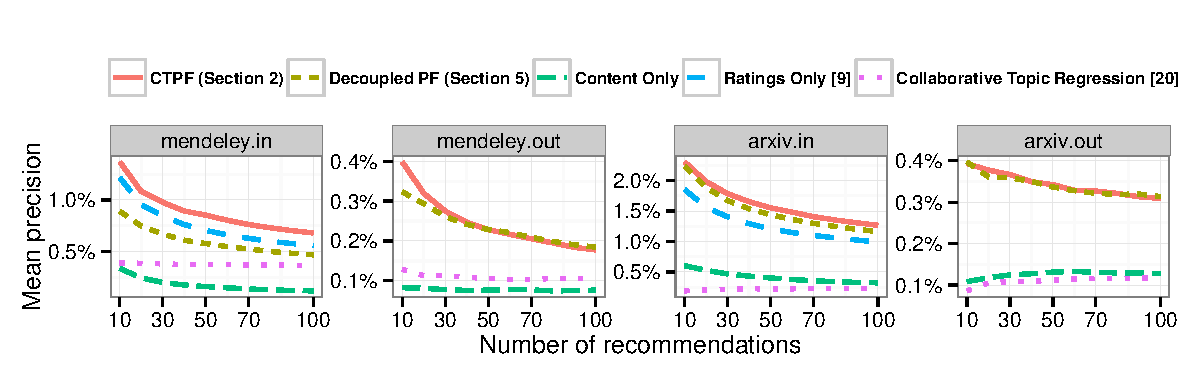
\includegraphics[width=0.95\textwidth]{../fig/pdf/mean_precision_by_num_recs.pdf}
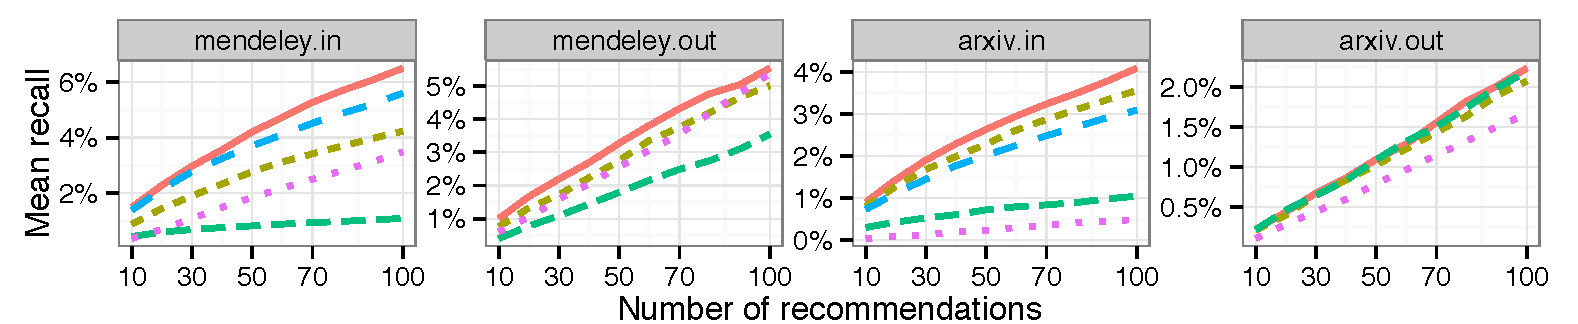
\includegraphics[width=0.94\textwidth]{../fig/pdf/mean_recall_by_num_recs.pdf}\\
\caption{
\footnotesize{The CTPF coordinate ascent algorithm outperforms CTR and
  other competing algorithms on both in-matrix and out-matrix
  predictions. Each panel shows the in-matrix or out-matrix
  recommendation task on the Mendeley data set or the 1-year arXiv
  data set. Note that the Ratings-only model cannot make out-matrix
  predictions. The mean precision and mean recall are computed from a
  random sample of 10,000 users.}}
\label{fig:precision_recall_at_20}
\vspace{-0.6cm}
\end{figure*}

\paragraph{Competing methods.} We study the predictive performance of the
following models. With the exception of the Poisson
factorization~\cite{Gopalan:2013b}, which does not model content, the
topics and topic intensities (or proportions) in all CTPF models are
initialized using LDA~\cite{Blei:2003b}, and fit using batch
variational inference. We set $K=100$ in all of our experiments.

\begin{itemize}
\item {\bf CTPF}: CTPF is our proposed model (\mysec{model}) with
  latent user preferences tied to a single vector $\eta_u$, and
  interpreted as affinity to latent topics $\beta$.

\item {\bf Decoupled Poisson Factorization}: This model is similar to
  CTPF but decouples the user latent preferences into distinct
  components $p_u$ and $q_u$, each of dimension $K$. We have,
\begin{align}
w_{dv} \sim \Pois(\theta_d^T \beta_v); \quad  r_{ud} \sim \Pois(p_u^T\theta_d + q_u^T\epsilon_d).  
\label{eq:decoupled} 
\end{align}
The user preference parameters for content and ratings can vary
freely.  The $q_u$ are independent of topics and offer greater
modeling flexibility, but they are less interpretable than the
$\eta_u$ in CTPF. Decoupling the factorizations has been proposed
by~\citet{Porteous:2010}.

\item {\bf Content Only}: We use the CTPF model without the document
  topic offsets $\epsilon_d$. This resembles the idea developed
  in~\cite{Agarwal:2010} but using Poisson generating distributions.

\item {\bf Ratings Only~\cite{Gopalan:2013b}}: We use Poisson
  factorization to the observed ratings. This model can only make
  in-matrix predictions.

\item {\bf CTR~\cite{Wang:2011a}}: A full optimization of this model
  does not scale to the size of our data sets despite running for
  several days. Accordingly, we fix the topics and document topic
  proportions to their LDA values. This procedure is shown to perform
  almost as well as jointly optimizing the full model
  in~\cite{Wang:2011a}. We follow the authors' experimental settings.
  Specifically, for hyperparameter selection we started with the
  values of hyperparameters suggested by the authors and explored
  various values of the learning rate as well as the variance of the
  prior over the correction factor ($\lambda_v$
  in~\cite{Wang:2011a}). Training convergence was assessed using the
  model's complete log-likelihood on the training observations. (CTR
  does not use a validation set.)
\end{itemize}

\begin{figure*}[t]
\centering
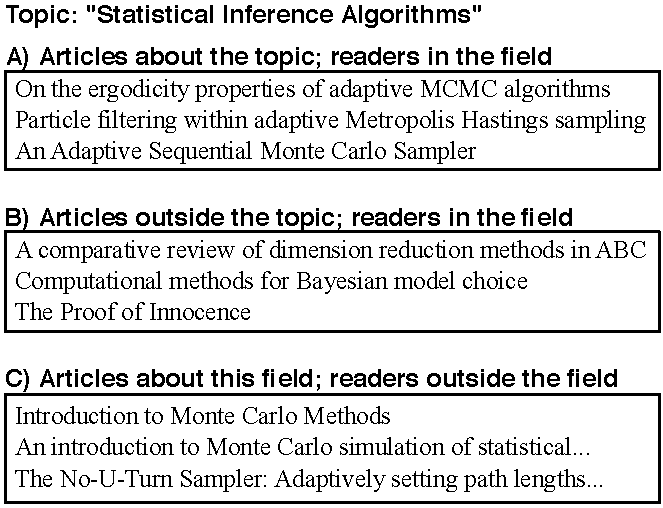
\includegraphics[width=0.49\textwidth]{../fig/pdf/arxiv-exploratory.pdf}
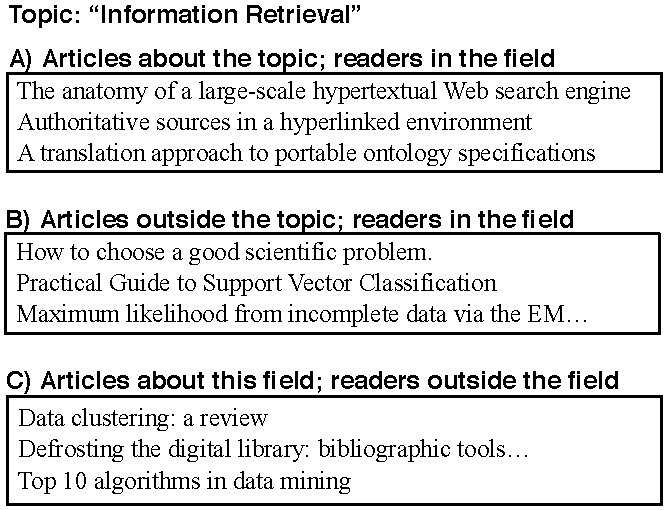
\includegraphics[width=0.49\textwidth]{../fig/pdf/mendeley-exploratory.pdf}
\caption{
\footnotesize{
The top articles by the expected
weight $\theta_{dk}$ from a component discovered by our stochastic
variational inference in the arXiv data set (Left) and Mendeley (Right).
Using the expected topic
proportions $\theta_{dk}$ and the expected topic offsets $\epsilon_{dk}$,
we identified subclasses of articles: A) corresponds
to the top articles by topic proportions in the field of ``Statistical
inference algorithms'' for arXiv and ``Ontologies and applications'' for Mendeley; B) corresponds to the top
articles with low topic proportions in this field, but a large
$\theta_{dk} + \epsilon_{dk}$, demonstrating the outside interests of
readers of that field (e.g., very popular papers often appear such as
``The Proof of Innocence'' which describes a rigorous way to ``fight your
traffic tickets''). 
C)  corresponds to the top articles with high topic proportions in this
field but that also draw significant interest from outside readers. }}
\label{fig:arxiv-exploratory}
\vspace{-0.5cm}
\end{figure*}

\paragraph{Evaluation.} Prior to training models, we randomly select 20\% of
ratings and 1\% of documents in each data set to be used as a held-out
test set. Additionally, we set aside 1\% of the training ratings as a
validation set (20\% for arXiv) and use it to determine
convergence. We used the CTPF settings described in \mysec{inference}
across both data sets. During testing, we generate the top $M$
recommendations for each user as those items with the highest
predictive score under each method.
\myfig{precision_recall_at_20} shows the mean precision and mean
recall at varying number of recommendations for each method and data
set. We see that CTPF outperforms CTR and the Ratings-only model on
all data sets. CTPF outperforms the Decoupled PF model and the
Content-only model on all data sets except on cold-start predictions
on the arXiv data set, where it performs equally well. The Decoupled
PF model lacks CTPF's interpretable latent space. The Content-only
model performs poorly on most tasks; it lacks a corrective term on
topics to account for user ratings. In \myfig{arxiv-exploratory}, we
explored the Mendeley and the arXiv data sets using CTPF. We fit the
Mendeley data set using the coordinate ascent algorithm, and the full
arXiv data set using the stochastic algorithm from \mysec{inference}.
Using the expected document topic intensities $\theta_{dk}$ and the
expected document topic offsets $\epsilon_{dk}$, we identified
interpretable topics and subclasses of articles that reveal the
interaction patterns between readers and articles.



\small{
\bibliographystyle{plainnat}
\begin{thebibliography}{25}
\providecommand{\natexlab}[1]{#1}
\providecommand{\url}[1]{\texttt{#1}}
\expandafter\ifx\csname urlstyle\endcsname\relax
  \providecommand{\doi}[1]{doi: #1}\else
  \providecommand{\doi}{doi: \begingroup \urlstyle{rm}\Url}\fi

\bibitem[Agarwal and Chen(2010)]{Agarwal:2010}
D.~Agarwal and B.~Chen.
\newblock f{LDA}: Matrix factorization through latent {D}irichlet allocation.
\newblock In \emph{Proceedings of the third ACM international conference on web
  search and data mining}, pages 91--100. ACM, 2010.

\bibitem[Amari(1982)]{Amari:1982}
S.~Amari.
\newblock Differential geometry of curved exponential families-curvatures and
  information loss.
\newblock \emph{The Annals of Statistics}, 10\penalty0 (2):\penalty0 357--385,
  1982.

\bibitem[Blei et~al.(2003)Blei, Ng, and Jordan]{Blei:2003b}
D.~Blei, A.~Ng, and M.~Jordan.
\newblock latent {D}irichlet allocation.
\newblock \emph{Journal of Machine Learning Research}, 3:\penalty0 993--1022,
  January 2003.

\bibitem[Canny(2004)]{Canny:2004}
J.~Canny.
\newblock {G}a{P}: {A} factor model for discrete data.
\newblock In \emph{Proceedings of the 27th Annual International ACM SIGIR
  Conference on Research and Development in Information Retrieval}, 2004.

\bibitem[Cemgil(2009)]{Cemgil:2009}
A.~Cemgil.
\newblock Bayesian inference for nonnegative matrix factorization models.
\newblock \emph{Computational Intelligence and Neuroscience}, 2009.

\bibitem[Dempster et~al.(1977)Dempster, Laird, and Rubin]{Dempster:1977}
A.~Dempster, N.~Laird, and D.~Rubin.
\newblock Maximum likelihood from incomplete data via the {EM} algorithm.
\newblock \emph{Journal of the Royal Statistical Society, Series B},
  39:\penalty0 1--38, 1977.

\bibitem[Dunson and Herring(2005)]{Dunson:2005}
D.~B Dunson and A.~H. Herring.
\newblock Bayesian latent variable models for mixed discrete outcomes.
\newblock \emph{Biostatistics}, 6\penalty0 (1):\penalty0 11--25, 2005.

\bibitem[Geisser and Eddy(1979)]{Geisser:1979}
S.~Geisser and W.F. Eddy.
\newblock A predictive approach to model selection.
\newblock \emph{Journal of the American Statistical Association}, pages
  153--160, 1979.

\bibitem[Ghahramani and Beal(2000)]{Ghahramani:2000}
Z.~Ghahramani and M.~Beal.
\newblock Variational inference for {B}ayesian mixtures of factor analysers.
\newblock In \emph{Neural Information Processing Systems}, volume~12, 2000.

\bibitem[Gopalan et~al.(2013)Gopalan, Hofman, and Blei]{Gopalan:2013b}
P.~Gopalan, J.M. Hofman, and D.~Blei.
\newblock Scalable recommendation with {P}oisson factorization.
\newblock \emph{arXiv preprint arXiv:1311.1704}, 2013.

\bibitem[Hoffman et~al.(2010)Hoffman, Blei, and Bach]{Hoffman:2010a}
M.~Hoffman, D.~Blei, and F.~Bach.
\newblock On-line learning for latent {D}irichlet allocation.
\newblock In \emph{Neural Information Processing Systems}, 2010.

\bibitem[Hoffman et~al.(2013)Hoffman, Blei, Wang, and Paisley]{Hoffman:2013}
M.~Hoffman, D.~Blei, C.~Wang, and J.~Paisley.
\newblock Stochastic variational inference.
\newblock \emph{Journal of Machine Learning Research}, 14:\penalty0 1303--1347,
  2013.

\bibitem[Hong et~al.(2013)Hong, Doumith, and Davison]{Hong:2013}
L.~Hong, A.~S. Doumith, and B.D. Davison.
\newblock Co-factorization machines: {M}odeling user interests and predicting
  individual decisions in {T}witter.
\newblock In \emph{Proceedings of the sixth ACM international conference on web
  search and data mining}, pages 557--566. ACM, 2013.

\bibitem[Hu et~al.(2008)Hu, Koren, and Volinsky]{Hu:2008}
Y.~Hu, Y.~Koren, and C.~Volinsky.
\newblock Collaborative filtering for implicit feedback datasets.
\newblock In \emph{Eighth IEEE International Conference on Data Mining.}, pages
  263--272. IEEE, 2008.

\bibitem[Jack et~al.(2010)Jack, Hammerton, Harvey, Hoyt, Reichelt, and
  Henning]{Jack:2010}
K.~Jack, J.~Hammerton, D.~Harvey, J.~J. Hoyt, J.~Reichelt, and V.~Henning.
\newblock Mendeley's reply to the datatel challenge.
\newblock \emph{Procedia Computer Science}, 1\penalty0 (2):\penalty0 1--3,
  2010.
\newblock URL \url{http://www.mendeley.com/research/sei-whale/}.

\bibitem[Johnson et~al.(2005)Johnson, Kemp, and Kotz]{Johnson:2005}
N.~Johnson, A.~Kemp, and S.~Kotz.
\newblock \emph{Univariate Discrete Distributions}.
\newblock John Wiley \& Sons, 2005.

\bibitem[Jordan et~al.(1999)Jordan, Ghahramani, Jaakkola, and
  Saul]{Jordan:1999}
M.~Jordan, Z.~Ghahramani, T.~Jaakkola, and L.~Saul.
\newblock Introduction to variational methods for graphical models.
\newblock \emph{Machine Learning}, 37:\penalty0 183--233, 1999.

\bibitem[Porteous et~al.(2010)Porteous, Asuncion, and Welling]{Porteous:2010}
I.~Porteous, A.~U. Asuncion, and M.~Welling.
\newblock Bayesian matrix factorization with side information and {D}irichlet
  process mixtures.
\newblock In Maria Fox and David Poole, editors, \emph{In the conference of the
  Association for the Advancement of Artificial Intelligence}. AAAI Press,
  2010.

\bibitem[Robbins and Monro(1951)]{Robbins:1951}
H.~Robbins and S.~Monro.
\newblock A stochastic approximation method.
\newblock \emph{The Annals of Mathematical Statistics}, 22\penalty0
  (3):\penalty0 400--407, 1951.

\bibitem[Salakhutdinov and Mnih(2008)]{Salakhutdinov:2008}
R.~Salakhutdinov and A.~Mnih.
\newblock Bayesian probabilistic matrix factorization using {M}arkov chain
  {M}onte {C}arlo.
\newblock In \emph{Proceedings of the 25th international conference on machine
  learning}, pages 880--887, 2008.

\bibitem[Shan and Banerjee(2010)]{Shan:2010}
H.~Shan and A.~Banerjee.
\newblock Generalized probabilistic matrix factorizations for collaborative
  filtering.
\newblock In \emph{Data Mining (ICDM), 2010 IEEE 10th International Conference
  on}, pages 1025--1030. IEEE, 2010.

\bibitem[Singh and Gordon(2008)]{Singh:2008}
A.~P. Singh and G.~J. Gordon.
\newblock Relational learning via collective matrix factorization.
\newblock In \emph{Proceedings of the 14th ACM SIGKDD international conference
  on Knowledge discovery and data mining}, pages 650--658. ACM, 2008.

\bibitem[Wang and Blei(2011)]{Wang:2011a}
C.~Wang and D.~Blei.
\newblock Collaborative topic modeling for recommending scientific articles.
\newblock In \emph{Knowledge Discovery and Data Mining}, 2011.

\bibitem[Wang et~al.(2011)Wang, Paisley, and Blei]{Wang:2011}
C.~Wang, J.~Paisley, and D.~Blei.
\newblock Online variational inference for the hierarchical {D}irichlet
  process.
\newblock In \emph{Artificial Intelligence and Statistics}, 2011.

\bibitem[Zhang and Carin(2012)]{Zhang:2012}
X.~Zhang and L.~Carin.
\newblock Joint modeling of a matrix with associated text via latent binary
  features.
\newblock In \emph{Advances in Neural Information Processing Systems}, pages
  1556--1564, 2012.

\end{thebibliography}

}

 % supplementary.tex
\section{Stochastic variational inference for the collaborative topic Poisson
  factorization model}
Stochastic variational inference combines stochastic gradient algorithms and
variational inference~\cite{Hoffman:2013}. Stochastic gradient algorithms
follow noisy estimates of the gradient with a decreasing step-size. If the
expectation of the noisy gradient equals to the gradient and if the step-size
decreases according to a certain schedule, then the algorithm converges to a
local optimum~\cite{Robbins:1951}. To obtain noisy gradients, assume that we
operate under the setting where we subsample a single document $d$ uniformly at
random from the $D$ documents. This sampling strategy is similar to online
LDA~\cite{Hoffman:2010a}. However, our approach differs in the use of separate
learning rates for each user, allowing the inference to update only the
relevant users in each iteration.

We are given observations about a single document in each iteration.  Following
~\cite{Hoffman:2013}, we use the conditional dependencies in our graphical
model to divide our variational parameters into \emph{local} and
\emph{global}. The multinomial parameters $(\phi_{dv}, \xi_{ud})$ for the
sampled document $d$ and for all $u \in U$, and the Gamma parameters for
$(\theta_{dk}, \epsilon_{dk})$ are local. All other varational parameters are
global.

In each iteration of our algorithm, we first subsample a document. We then
update the local multinomial parameters and the local topic intensities and
offset parameters for this document using the coordinate updates from
Figure 2. 
This optimizes the local parameters with respect to the
subsample. We then compute scaled natural gradients~\cite{Amari:1982} for the
global user preference parameters $(\vshape{\eta}{uk}, \vrate{\eta}{uk})$ for the
users $u$ that have rated document $d$ and for all topic parameters
$(\vshape{\beta}{vk}, \vrate{\beta}{vk})$. The global step for the global
parameters follows the noisy gradient with an appropriate step-size. 

We maintain separate learning rates $\rho_u$ for each user, and only update the
users who have rated the document $d$. We proceed similarly for words. We maintain a global learning rate
$\rho'$ for the topic parameters, which are updated in each iteration.  For
each of these learning rates $\rho$, we require that $\sum_{t} \rho(t)^2 <
\infty$ and $\sum_{t} \rho(t) = \infty$ for convergence to a local
optimum~\citep{Robbins:1951}. We set $\rho(t) = (\tau_0 + t)^{-\kappa}$, where
$\kappa \in (0.5,1]$ is the learning rate and $\tau_0 \geq 0$ downweights early
  iterations~\cite{Hoffman:2013}. 

\begin{figure}
\begin{center}
 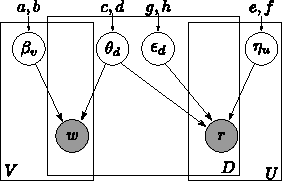
\includegraphics{../fig/pdf/graphical_model}
 \caption{The collaborative topic Poisson factorization model (CTPF).}
 \label{fig:graphical_model}
 \end{center}
\end{figure}



\end{document}
